\documentclass[journal]{IEEEtran}
\ifCLASSINFOpdf
\else
\fi
\usepackage{cite}
\usepackage[cmex10]{amsmath}
\usepackage{amssymb}
\usepackage{algorithmic}
\usepackage{array}
\usepackage{mdwmath}
\usepackage{booktabs}
\usepackage{mdwtab}
\usepackage{eqparbox}
\usepackage{graphicx}
\usepackage[justification=centering]{caption}
\usepackage{bm}
\usepackage{float}
\usepackage [latin1]{inputenc}
%\fnbelowfloat
%\ifCLASSOPTIONcaptionsoff
%  \usepackage[nomarkers]{endfloat}
% \let\MYoriglatexcaption\caption
% \renewcommand{\caption}[2][\relax]{\MYoriglatexcaption[#2]{#2}}
%\fi
% \let\MYorigsubfloat\subfloat
% \renewcommand{\subfloat}[2][\relax]{\MYorigsubfloat[]{#2}}
% \let\MYorigsubfigure\subfigure
% \renewcommand{\subfigure}[2][\relax]{\MYorigsubfigure[]{#2}}
%\usepackage{url}
\hyphenation{optical networks semiconductor}
\begin{document}
\title{ Classification and Multi-objective Optimization of Decompressed ECG Signals  }

\author{

\thanks{%Manuscript received April 19, 2013; revised January 11, 2007.
This work is supported by the National Natural Science Foundation of China under Grant 11404113, and the Guangzhou Key Laboratory of Brain Computer Interaction and Applications under Grant 201509010006. \textit{Corresponding
author: Wei Cui.}

The authors are with the School of Automation Science and Engineering, South China University of Technology, Guangzhou 510641, China~(e-mails: 852934033@qq.com, aucuiwei@scut.edu.cn, wangcong@scut.edu.cn).
}}
%\thanks{This work is supported by the National Natural Science Foundation of China under Grant 11404113, and the Guangzhou Key Laboratory of Brain Computer Interaction and Applications under Grant 201509010006.
%\textit{Corresponding author: Wei Cui.}}
%\thanks{W. Cui is with Quantum Condensed Matter Research Group (QCMG),  Center for Emergent Matter Science (CEMS), Institute of Physics and Chemical Research (RIKEN), Saitama, 351-0198, Japan (e-mail: wcui@riken.jp).}
%\thanks{F. Nori is with Quantum Condensed Matter Research Group (QCMG),  Center for Emergent Matter Science (CEMS), Institute of Physics and Chemical Research (RIKEN), Saitama, 351-0198, and also with Physics Department, The University of Michigan, Ann Arbor, Michigan 48109-1040, USA (e-mail: fnori@riken.jp, see http://dml.riken.jp/index.php).}}

%\hfill mds
%\hfill January 11, 2007
\markboth{Submitted to IEEE Journal of Biomedical and Health Informatics}
{Shell \MakeLowercase{\textit{et al.}}: Bare Demo of IEEEtran.cls for Journals}
\maketitle
\IEEEpeerreviewmaketitle

\begin{abstract}
 Electrocardiogram (ECG) monitoring systems are widely applied to tele-cardiology healthcare programs nowadays, where ECG signal must be compressed first during its transmission and storage. Unlike previous studies which placed as prior as well as attempted to achieve a decompressed signal with extremely high quality while increasing the compression ratio as high as possible, we aimed at investigating that the decompressed signal with a considerable distortion after the lossy compression with a high compression ratio can still work well in ECGs classification. This paper utilized singular value decomposition to decompose ECGs, then applied the decompressed data into the CNN and SVM classification model. Using the optimization method with accuracy and compression ratio as objective functions, the highest average accuracy which is above 96\% can be achieved when the singular value equals 3. The experimental results demonstrated that, due to the characteristics of ECGs and a wise optimized strategy, the decompressed ones even with a relatively high distortion can still achieve a satisfying performance in the classification of ECGs.
\end{abstract}

\section{Introduction}
\IEEEPARstart{I}{n} modern society, the number of people dying from cardiovascular disease each year is the main cause of abnormal human death and has been growing at an alarming rate. Remote ECG monitoring system, ECG monitoring mobile phone terminal, hospital monitoring center server and network communication support are widely used in medical treatment. With the collected electrocardiogram signals, patient's cardiac health condition is able to be monitored and classified [1-5] in real time under the ECG telemetry systems, and medical professionals can react much more promptly and efficiently to some acute cardiac diseases, making the transmission of ECG signals an indispensable and essential part of the whole procedure. However, due to multiple cycles and high resolution, the amount of collected ECG data is so large that negatively affected the transmission efficiency and portability of ECG data, thus calling for the compression of ECG signals. Figure 1 is a schematic diagram of an ECG monitoring system. The ECG signal is obtained through a wearable electronic device of the terminal, and compressed then transmitted to a server for decompression and signal classification.

\begin{figure}[H]
	\centering
	% Requires \usepackage{graphicx}
	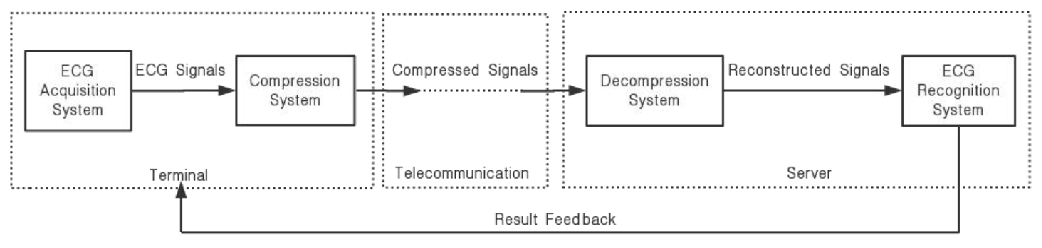
\includegraphics[width=10cm]{SysModel.pdf}\\
	\caption{ECG signal[28]}
	\label{Doc1}
\end{figure}

In the past few decades, researchers have devoted plenty of efforts into the field regarding compression and proposed a myriad of methods to achieve better performances, which are divided into lossy and lossless ones. Lossy compressions are often used in ECG signal compression due to its high compression ratio (CR). A comparison and investigation about earlier work can be found in the paper [6]. In general, ECG signal compression techniques can be divided into three types. The basic idea of the first one is to detect redundancy and compress the ECG signals in the time domain, like amplitude zone time epoch coding (AZTEC) [7], scan along polygonal approximation (SAPA) [8], and the coordinate reduction time encoding system (CORTES) [9]. The second method is aimed at extracting and coding particular parameters and features of ECG signals, such as linear prediction method [10], the neural network method [11], and vector quantization [12] and so on. The third method is to analyze the energy distribution by transforming ECG signals from time domain to frequency or other domains; for example, the Fourier transform [13], Karhunen-Loeve transform (KLT) [14], the discrete cosine transform (DCT) [15], the wavelet transform [16], and the singular value decomposition (SVD) [17][18]. Mostly every researcher is dedicated to design a better way of compression and seek for a balance to optimize the compression performance between high compression ratio and high quality of reconstruction without compromising either of them. However, while advancing the lossless compression algorithm, researchers have overlooked the promising superiority of lossy compression in practical applications, since there is every likelihood that the performance in some particular application is slightly influenced by the degree of loss in compression.

In order to ensure the accuracy of the diagnostic results, lossless compression is often used in the field of ECG monitoring and diagnosis, inevitably leading to a lower transmission efficiency [19]. We wonder whether a lossy compression, which can compress data more significantly at higher compression ratios than lossless compression, can create lost information in large amount to improve transmission efficiency without compromising the diagnostic accuracy. In fact, if the assumption is proved truth, the real-time nature of the remote mobile ECG monitoring system can be greatly improved and countless people who are in need of ECG diagnosis can benefit from it, which is why we write this paper. The rest of the paper is arranged as follows. The main features of ECG signal as well as the basic principles and ideas of Singular Value Decomposition(SVD) and Convolutional Neural Network (CNN) are summarized in Section 2. Section 3 presents the procedure of SVD-based compression including period normalization, compression and reconstruction. In Section 4, the Convolutional Neural Network (CNN) and SVM method are adopted into ECG classification with the compressed signals, the experimental results of which has been evaluated and compared. Finally, Section 5 multi-objective optimization is carried out with Error Rate and Compression Ratio as objective functions and several optimal solutions of singular values are obtained under different weights.

\section{Basic Signals and Methods}
\subsection{ECG}
The electrocardiogram(ECG) signals [20][21] play an important role in arrhythmia detection and classification, but when using manual analysis by a general physician it is quite time-consuming and possibly makes considerable mistakes at the same time, which calls for a highly accurate automatic classification method. In addition, automatic classification will be helpful to paramedical and emergency medical staff in cases where immediate action is required.

As shown in Figure 1, a typical one-cycle ECG waveform consists of P wave, QRS complex and T wave which are separated by intervals and segments. The horizontal portion prior to the P wave is referred as the baseline. P-wave is the first upward deflection with positive polarity that represents to the depolarization of the atrial musculature and has a duration of 80-110 ms. The three waves of the QRS complex, with the duration between 60 and 100 ms, corresponds to the combined result of the repolarization of the atria and depolarization of the ventricles. Q wave is the first downward deflection and R wave, as the largest wave, is always the first upward deflection after the Q wave while S wave is the negative one that immediately follows the R wave. Ventricular relaxation follows repolarization of the ventricles and is represented by T wave whose direction is consistent with QRS complex.


\begin{figure}[H]
	\centering
	% Requires \usepackage{graphicx}
	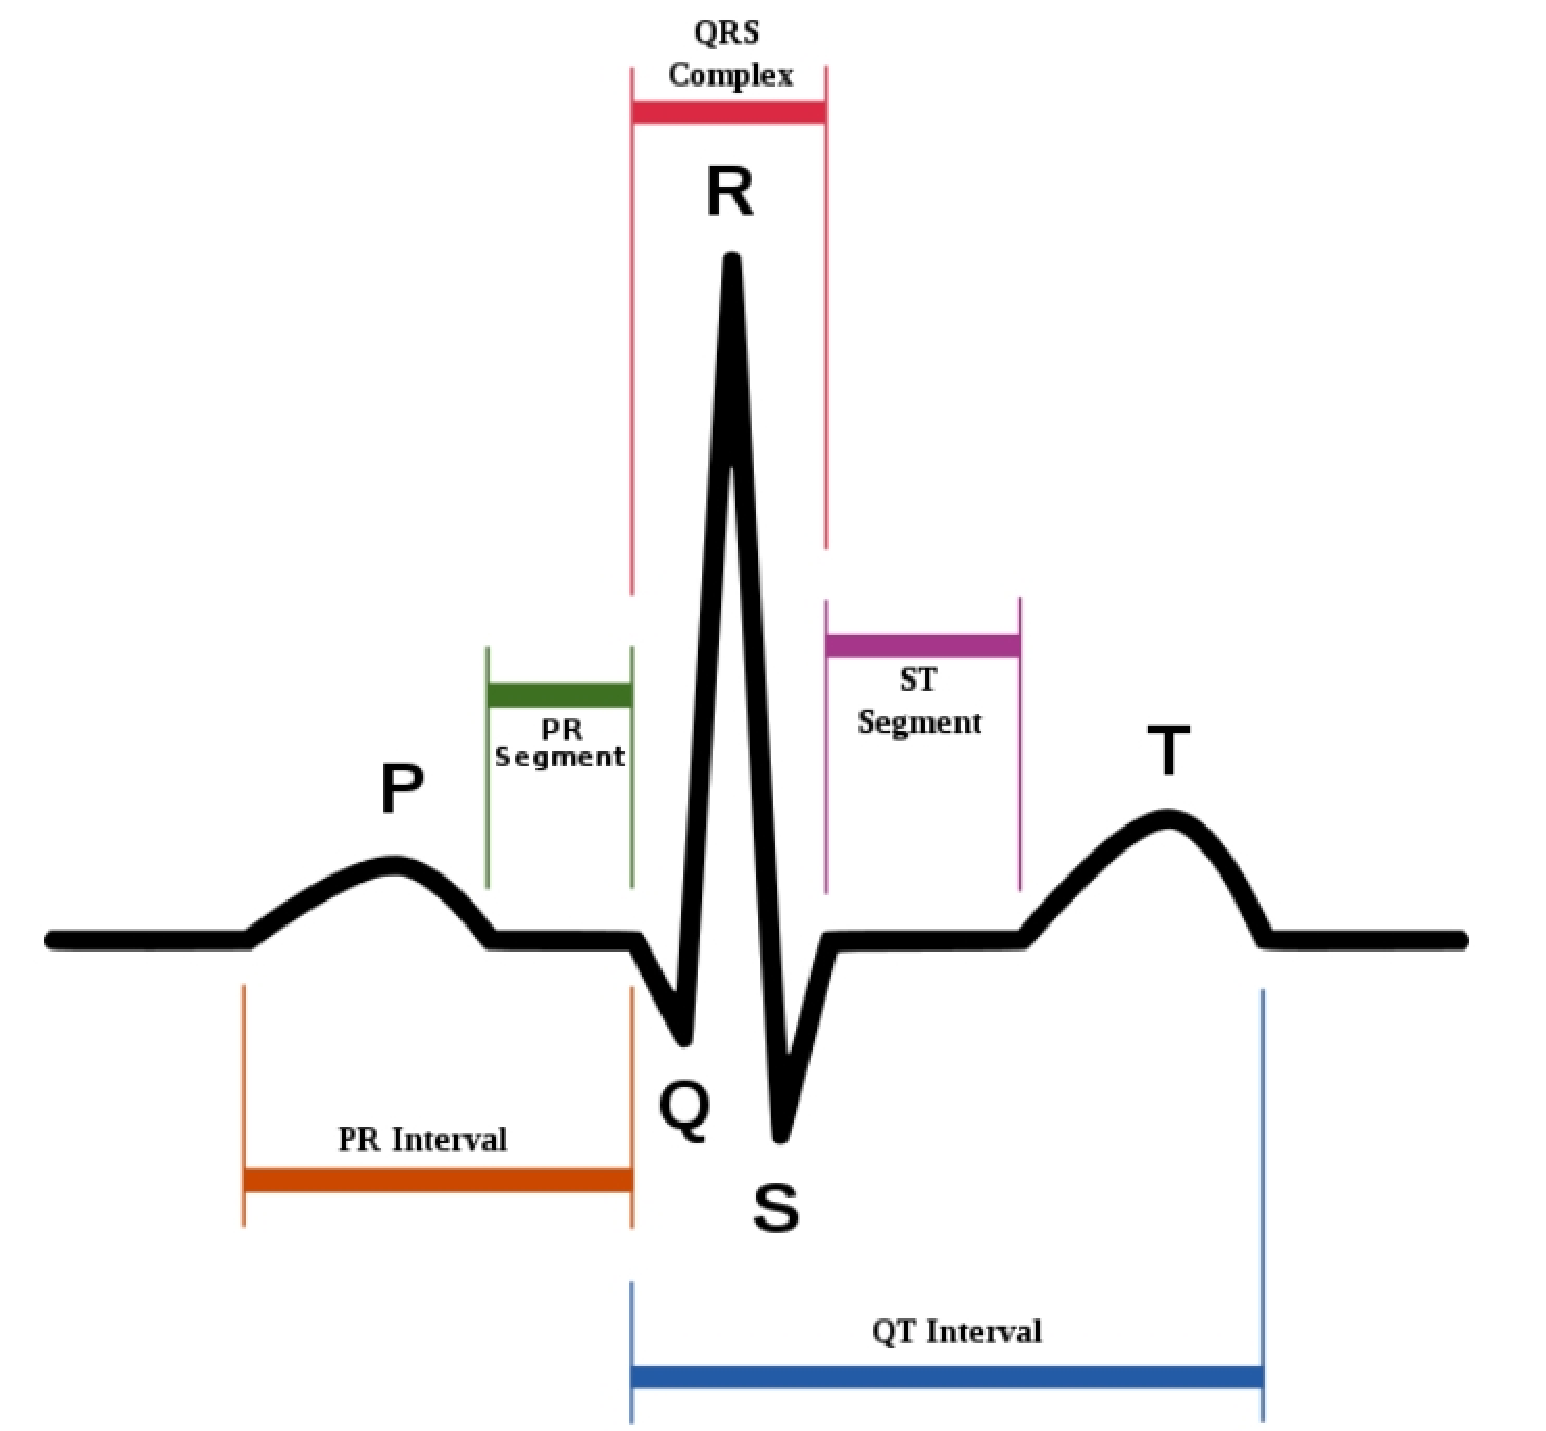
\includegraphics[width=6cm]{ecg.pdf}\\
	\caption{ECG signal[28]}
	\label{Doc1}
\end{figure}

The ECG signals used in this experiment are selected from MIT-BIH cardiac arrhythmia database [22] which is the most widely used database in recent years. MIT-BIH  database was provided by the Massachusetts Institute of Technology for the study of cardiac arrhythmias, containing 48 records, each slightly more than 30 minutes and sampled at 360 Hz.

The MIT-BIH database offers 13 different types of beats corresponding to each heart arrhythmia. To make ECG classification more accurate and monitoring result more comprehensive, four most common types of heart condition have been selected, including normal (N), left bundle branch block (LBBB), right bundle branch block (RBBB), ventricular premature beats (PVC). We define R peak is the marker point and each heartbeat contains the first 100 and the last 150 sampling points. Figure 2 is a schematic diagram of four types of sample beat.

%In order to perform classification on the compressed data, different heartbeat types of the compressed ECG signals need to be sorted into corresponding data set for later experiment. As shown in Figure 2, the label ``1'' denotes the heartbeat category ``normal'', label ``2'' suggests ``left bundle branch block'', label ``3'' stands for ``right bundle branch block'', and label ``5'' represents ``ventricular premature beat''. The above four types of heart beats are selected and organized into four different data sets. Based on the QRS wave, we include 100 sample points forward and 150 sample points as a heart beat.

\begin{figure}[H]
	\centering
	% Requires \usepackage{graphicx}
	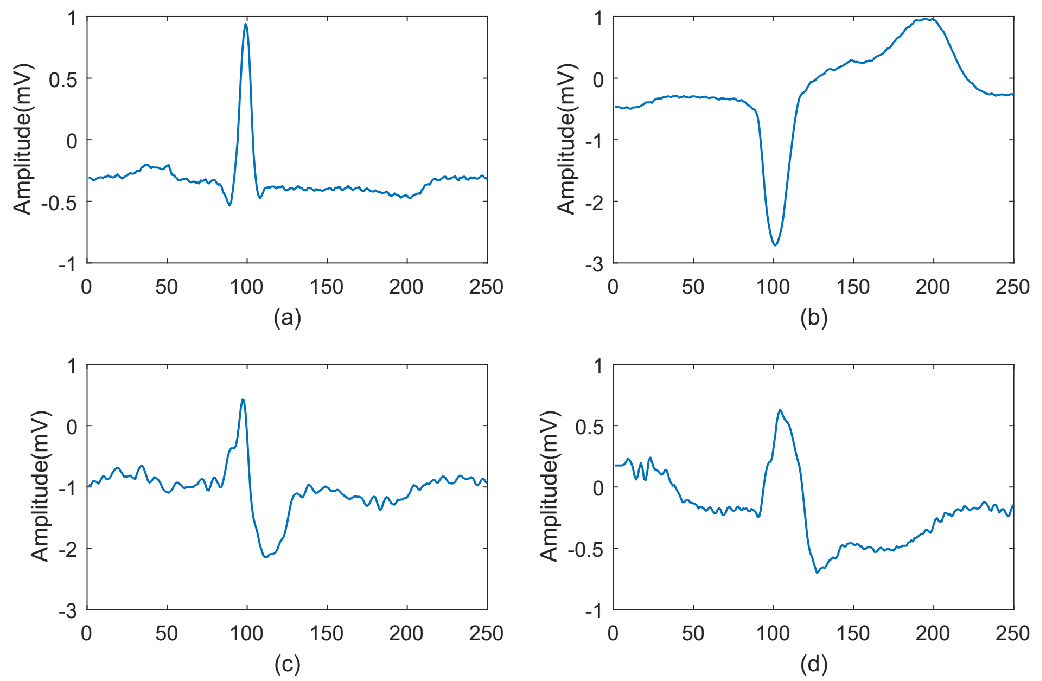
\includegraphics[width=9cm]{beat3.pdf}\\
	\caption{Four types of heart beat samples: (a) ``normal''(N); (b) ``ventricular premature beat''(PVC); (c) ``right bundle branch block''(RBBB); (d) ``left bundle branch block''(LBBB)}
	\label{Doc2}
\end{figure}


\subsection{SVD}
Since the signal processed by the singular value decomposition (SVD) technology is a periodic signal, if it is to be applied to the compression of the ECG signal, the ECG signal is normalized. During the normalization, the original ECG signal is divided into m R-to-R segments with a length n, via QRS peak detection [23]. Let $Y$ be the $m\times n$ matrix composed of the samples of the normalized ECG to be compressed, which can be described as follows:
\begin{equation}
Y
=\begin{bmatrix}
y_1(1)  &  y_1(2)  & \cdots\ &y_1(n)\\
y_2(1)  &  y_2(2)  & \cdots\ & y_2(n)\\
\vdots  & \vdots   & \ddots  & \vdots  \\
y_m(1)  & y_m(2)   & \cdots\ & y_m(n)\\
\end{bmatrix}
\end{equation}
The application of the SVD on the matrix Y yields $Y=U_y\sum_y(V_y)^T$, where $U_y=[u_1^y,\cdots,u_m^y]$, $V_y=[v_1^y,\cdots, v_n^y]$,$U_y^T U_y=I$, $V_y^T V_y=I$, and $\sum_y$ is a diagonal matrix whose diagonal entries are the singular values of Y in descending order. The matrix can be further performed by
\begin{equation}
Y=\sum\limits_{i=1}^{p}u_{i}^{y}\sigma_{i}^{y}(v_{i}^{y})^{T}
\end{equation}
where $p = min(m, n)$, $u_{i}^{y}$ and $v_{i}^{y}$ are the orthogonal eigenvectors of $YY^T$ and of $Y^TY$, respectively.

During the decompression process, in order to reduce the redundant data resulted from high correlation among ECG periodic signals, insignificant singular values can be truncated appropriately since information of the periodic signals is primarily focused on significant singular values representing the basic patterns and associated scaling vectors.

In the case of ideal ECGs, according to the decomposition process of SVD, except for the singular value representing the principal component, all other singular values will be zero, and the matrix will become a rank 1 matrix since it is a periodic signal with precise length. Therefore, only one singular value and associated eigenvector pairs are required for restoring the original signal unexceptionably.

However, in practical periodic physiological signals, ECG do not manifest perfect waveforms, both the periodic length and waveform pattern may show discrepancy to a certain extent. Therefore, in order to obtain the main information, $q$ predominant singular values need to be selected from $p$ and related vectors could be required to reconstruct ECG signals with a relatively high quality. Correspondingly, the above matrix Y can be reduced to the following form:
\begin{equation}
\hat Y=\sum\limits_{i=1}^{q}u_{i}^{y}\sigma_{i}^{y}(v_{i}^{y})^{T},q\leq p
\end{equation}

There are several commonly used indicators for judging the performance of compression algorithms, among which we choose\\
(1) Compression Rate(CR) which is the ratio of the number of bits required to store the original signal to that required to store the compressed signal, measuring the degree of data compression.
\begin{equation}
CR=\frac{bits~of~the~original~signals}{bits~of~the~compressed~signals}
%CR={bits of the original signals}{bits of the compressed signals}
\end{equation}
(2)Percent Root mean square Difference(PRD) which measures the error between the reconstructed signal and the original signal, that is, the quality of the reconstruction.
\begin{equation}
PRD=\sqrt{\frac{\sum\limits_{i=1}^{L}(x_0(i)-x_r(i))^2}{\sum\limits_{i=1}^{L}x_0(i)^2}} \times 100
\end{equation}
where $L$ is the number of sampling points.

(3)PRDN, the normalized version of PRD.
\begin{equation}
PRDN=\sqrt{\frac{\sum\limits_{i=1}^{L}(x_0(i)-x_r(i))^2}{\sum\limits_{i=1}^{L}(x_0(i)-\bar{x})^2}}\times 100
\end{equation}
(4)Root Mean Square error(RMS)that represents differences between signals' energy before and after the compression.
\begin{equation}
PRDN=\sqrt{\frac{1}{L} \cdot \sum\limits_{i=1}^{L}(x_0(i)-x_r(i))^2} \times 100
\end{equation}
(5)Quality Score(QS) considering both the compression ratio and the quality of the reconstructed signal, used to measure the overall performance of data compression. The higher the QS, the better the compression performance.
\begin{equation}
QS=\frac{CR}{PRD}
\end{equation}

\subsection{CNN}
CNN is a special structure of feedforward neural network, generally consist of input layer, convolution layers, pooling layers, fully-connected layers and output layer. The convolution layers and the pooling layers implement feature extraction, and the fully- connected layers use the extracted features to achieve classification or regression.

%The convolution layer neurons are organized into various feature planes, each of which is connected to a local area of the upper layer of the feature surface with a set of weights, whicn means that the neurons in the convolutional layer and the feature planes in the input layer perform local connections [24]. The local weighted sum is then passed to a nonlinear function such as the ReLU function to obtain the output value of each neuron in the convolutional layer. The ReLU function is described as follows:
The convolution layer is composed of a plurality of feature maps, each of which is composed of a plurality of neurons. Taking a one-dimensional CNN as an example, the neurons of the convolutional layer are organized into various feature maps, and each neuron is connected to the region of the next feature map by a set of weights, that is, the neurons in the convolutional layer are locally connected to the feature map in its input layer [24]. In the same input feature map and the same output feature map, the weights of the CNN are shared. The output of the convolutional layer can be obtained by passing the weighted sum of the local regions to a nonlinear function such as the ReLu function. In the current CNN structure, the unsaturated nonlinear function Relu function is commonly used as the excitation function of the convolutional layer, because the ReLu function can solve the gradient explosion and gradient disappearance problem, and also accelerate the convergence speed. The ReLU function is described as follows:

\begin{equation}
y=\max(0,x)
\end{equation}

%Similar to the convolutional layer, pooling layer is also composed of a plurality of feature planes, each of which is uniquely corresponding to and remains the same number as that of the upper layer. Specifically, since the convolution layer is the input layer of the pooling layer which serves as a secondary extraction feature, each feature surface of the convolution layer uniquely relates to that of the pooling layer, and the neurons of the pooling layer are also connected to the local accepting domain of the input layer. Meanwhile, the locally accepted domains of different neurons do not overlap. There are two commonly used pooling methods used in the this field so far--the largest pooling and the mean pooling.
Similar to a convolutional layer, a pooled layer is also composed of multiple feature maps. The pooled layer follows the convolutional layer, and each of its feature maps corresponds to the feature surface of its upper layer, so the number of feature faces is not changed. As the input layer of the pooling layer, the convolution layer has a feature map that uniquely corresponds to a feature map in the pooling layer. The neurons of the pooling layer are also connected to the local accepting domain of the input layer, and the different neurons are locally accepted. Different neurons' local accepting domain do not overlap. The pooling layer aims at obtaining spatially invariant features by reducing the resolution of the feature planes, so the pooling layer functions as a secondary extraction feature. There are two commonly used pooling methods used in the this field so far--the largest pooling and the mean pooling.

The largest pooling is described as a certain point where the local receiving domain has the largest value, while the mean pooling is the mean value of all values in the locally accepted domain and the random pooling [25].

%In the CNN structure, after the convolutional layers and the pooling layers are connected with one or more fully-connected layers, each neuron of which is also fully connected to all neurons in the previous layers, and the role of which is to gather the local information to distinguish categories in the convolutional or pooled layers. The activating function of each neuron in the fully-connected layer mainly bases on the ReLU function for the performance improvement of the CNN network. After the output value from the last fully-connected layer is passed to an output layer, this layer, which also called as the softmax layer, can apply logistic regression for classification and is described as belows:
In the CNN structure, one or more fully-connected layers are connected after the convolutional layers and the pooling layers. Similar to Multi-Layer Perception (MLP), each neuron in the fully- connected layer is fully connected to all neurons in the previous layers, and the role of the fully- connected layer is to integrate local information used to distinguish categories in the convolutional or pooled layers. The activating function of each neuron in the fully connected layer mostly uses the ReLU function for the performance improvement of the CNN network. The output value in the last fully-connected layer is passed to an output layer, which can use softmax logistic regression for classification. This layer can also be called the softmax layer. The softmax function is described as below:

\begin{equation}
y=\sigma(z)_j = \frac{e^{z_j}}{\sum_{k=1}^{K}e^{z_k}}
\end{equation}

Generally, CNN's fully connected layer is similar to MLP structures, thus BP algorithm can also be adpoted as its training algorithm. The procedure of CNN is shown in Figure 3.
\begin{figure}[H]
	\centering
	% Requires \usepackage{graphicx}
	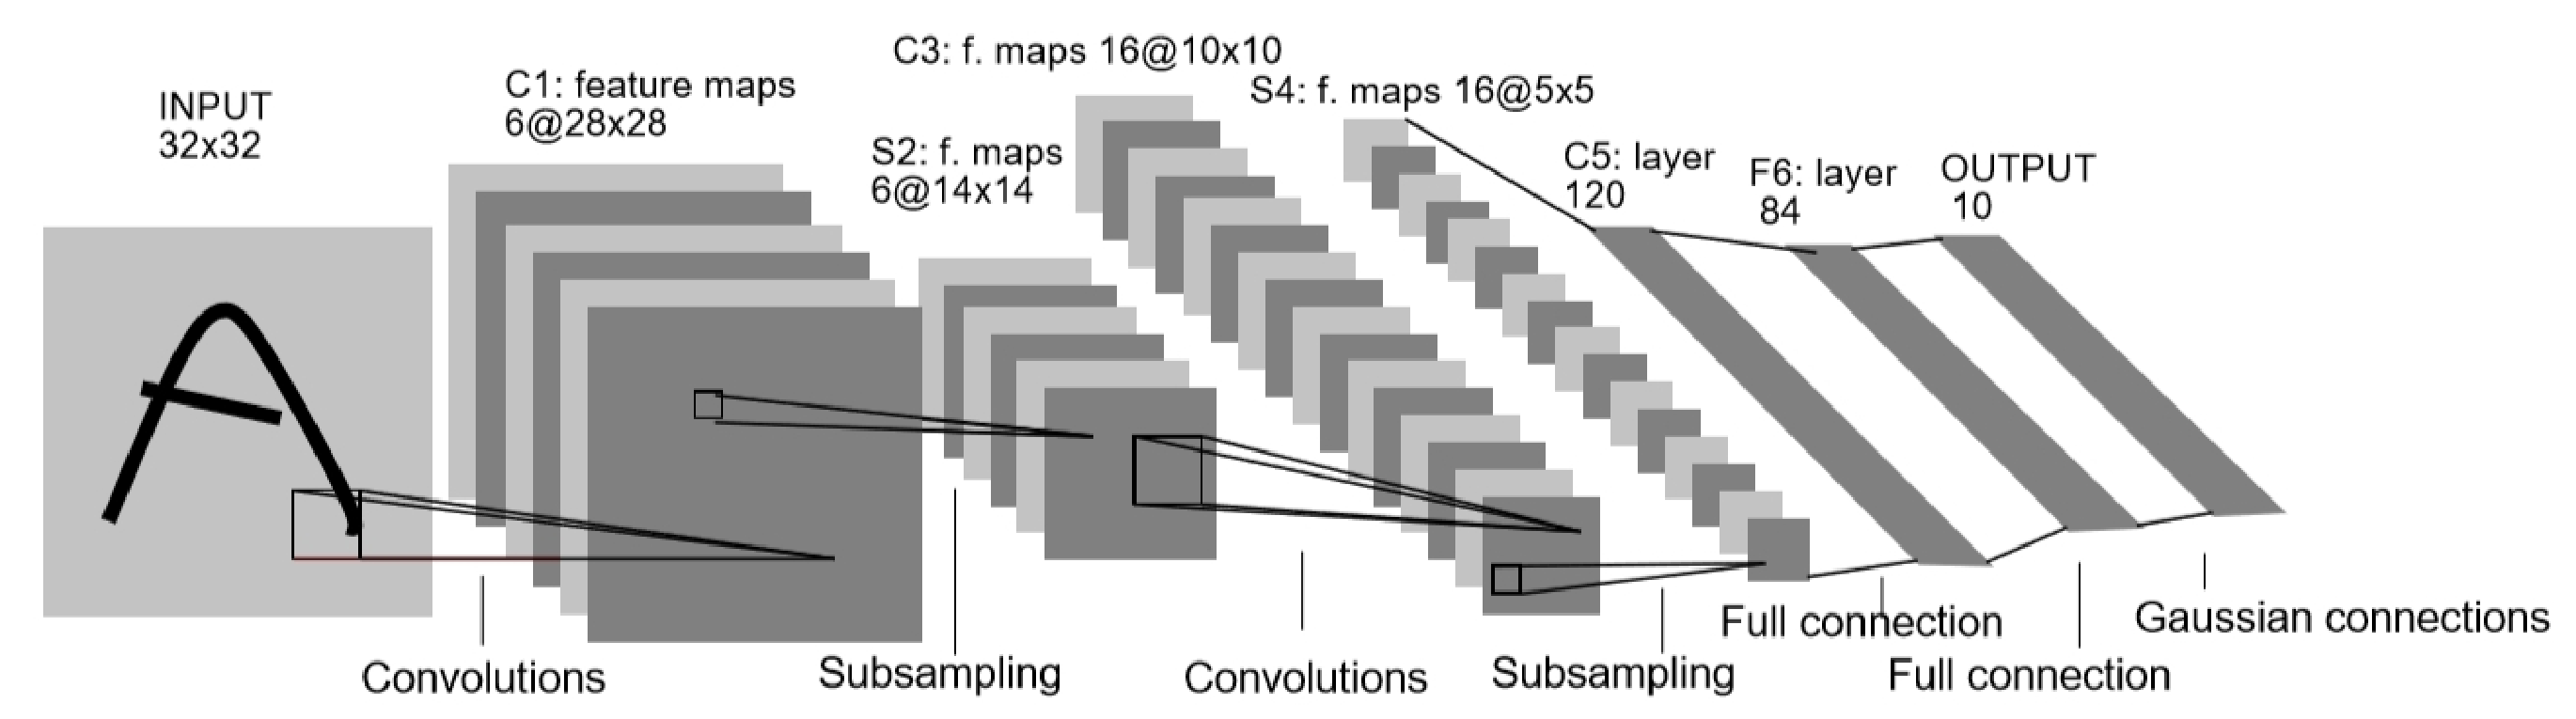
\includegraphics[width=9cm]{cnn.pdf}\\
	\caption{Structure of CNN[29]}
	\label{Doc5}
\end{figure}



\section{SVD-based Compression Procedure}
Figure 4 is a system diagram of the proposed ECG data SVD compression system. The ECG data is normalized by the period into a matrix $Y_{mn}$, and then the matrix is compressed using SVD. This will be described in more detail below along with the data reconstruction process.
\begin{figure}[H]
	\centering
	% Requires \usepackage{graphicx}
	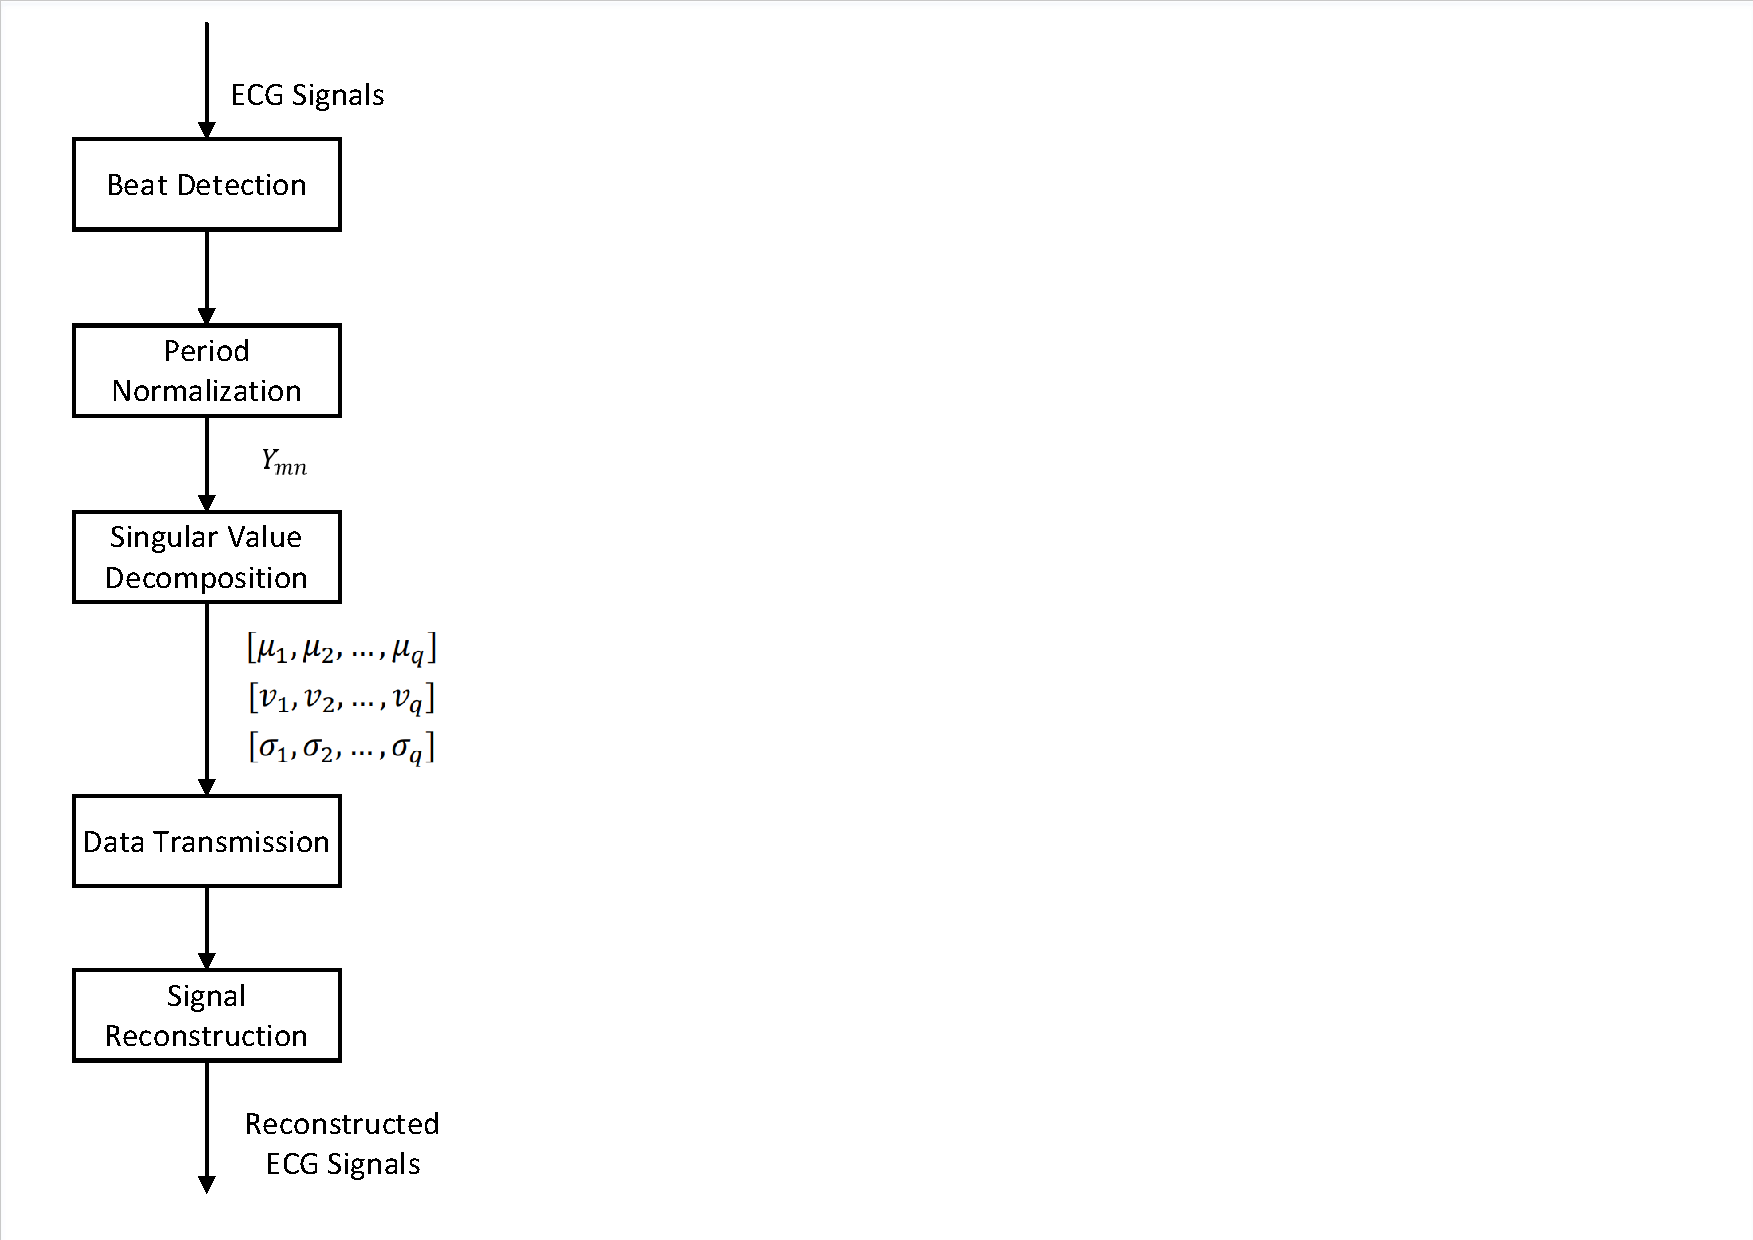
\includegraphics[width=14cm]{procedure.pdf}\\
	\caption{SVD compression and reconstruction procedure}
	\label{liuchengtu1}
\end{figure}


\subsection{Period Normalization}
Using the dual-slope processing [26] and low-pass filtering-based R-peak detection technique, it is possible to detect the R-peak and extract a segment between two consecutive R-peaks, that is, to cut out a single ECG cycle. However, since the extracted ECG cycles are not of equal length, periodic normalization is required to equalize them before applying SVD technique to compression. In previous work where the method of periodic normalization is mentioned, the lengths of all cycles are normalized to the average period length by separating a ECG signal into m cycles. The ith ECG segment can be presented as $x_i = [x_i(1), x_i(2), . . . , x_i(n)]$, where $n$ is the length of $x_i$, which can be converted to a segment $y_i = [y_i(1), y_i(2), . . . , y_i(n)]$ to simplify the calculation. In this way, the signal morphology of $x_i$ is identified with $y_i$'s while their lengths are not the same. The transformation is stated as follows:
\begin{equation}
y_i(j) = x_i(j) + (x_i(j+1)-x_i(j))(r_j-j)
\end{equation}

where $r_j=(j-1)*n/(n-1)+1$, $j$ is the integral part of $r_j$ .
Then, by placing each cycle as a row, the ECG signal is transformed to an $m*n$ matrix $Y_{mn}$.

\subsection{Compression and Reconstruction}
In practice, most of information is stored in the primary components of matrix, which can be used to recover  original signal with a high quality. By performing SVD method and determining the number of singular values, three matrices u, s, v are obtained, then the compressed signal can be reconstructed based on $Y'=s*u*v'$. Figure 5 is the comparison between the waveform of normalized and compressed ECG signals. From the comparison of the compressed and the decompression signals, it can be found that most information of ECG signals is preserved, especially that on the QRS complex. As for the rest of signals, though the waveforms are retained, they becomes slightly smoother.

\begin{figure}[H]
	\centering
	% Requires \usepackage{graphicx}
	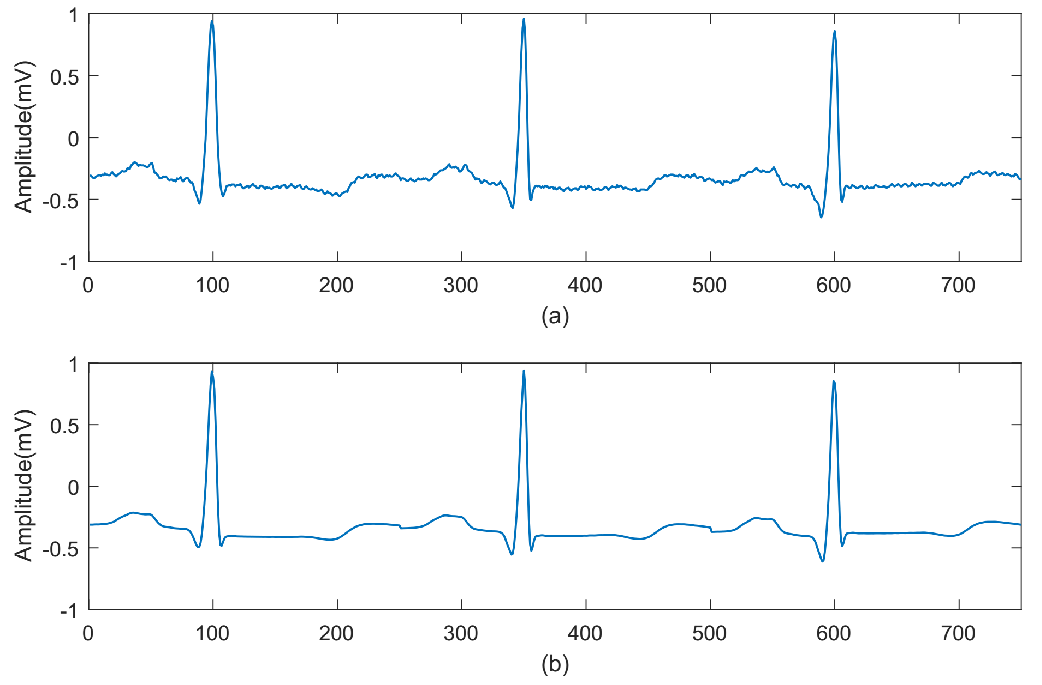
\includegraphics[width=9cm]{srcAndcompressBbeat3.pdf}\\
	\caption{Original and compressed ECG signals(record 100): (a) original signal; (b)compressed signal at $q$ = 5}
	\label{Doc2}
\end{figure}

 \begin{center}
	\scriptsize
	%\begin{threeparttable}
	{ Table~1\\ Results obtained for 11 records(q=5)}\\
	\label{tab:1} \vskip 3pt
    \newcommand{\rb}[1]{\raisebox{1.9ex}[-2pt]{#1}}
	\begin{tabular}{c|cccccc}
		\toprule
		Records & CR & PRD(\%) & PRDN(\%) & RMS & SNR & QS \\
		\midrule
		100  & 50.70 & 6.16 & 11.55 & 2.23 & 18.75 & 8.23 \\
		101  & 58.54 & 7.76 & 11.29 & 3.05 & 18.95 & 7.54 \\
		103  & 54.16 & 7.46 & 9.16  & 2.96 & 20.76 & 7.26 \\
		107  & 53.12 & 14.02& 14.53 & 12.47& 16.76 & 3.79 \\
		109  & 46.43 & 10.73& 11.83 & 5.87 & 18.54 & 4.33 \\
		111  & 53.39 & 13.77& 16.40 & 4.16 & 15.70 & 3.88 \\
		115  & 56.77 & 5.36 & 8.94  & 3.27 & 20.97 & 10.59\\
		117  & 66.15 & 3.39 & 12.43 & 3.01 & 18.11 & 19.49\\
		119  & 56.03 & 5.99 & 10.28 & 5.95 & 19.76 & 9.36 \\
		214  & 50.84 & 16.10& 17.03 & 7.99 & 15.37 & 3.16 \\
		223  & 45.38 & 10.81& 17.49 & 7.12 & 15.14 & 4.20 \\
		\midrule
   Averaged  & 53.77 & 9.23 & 12.81 & 5.28 & 18.07 & 5.83 \\
		\bottomrule
	\end{tabular}
\end{center}


Performances measured by the above indicators including CR, PRD(\%), PRDN(\%), RMS, SNR and QS in terms of values are sorted into the following table. As shown in the table, the average value of CR is 53.77 and its value can up to 66.15 in record 117, which demonstrates the considerable and satisfying compression ratio. However, when it comes to PRD(\%), the average value of which is only 9.23 and in the worst case, namely record 117, the is as low as 3.39, indicating that the quality of reconstructed signal is poor. However, our goal is to increase the compression ratio, so there is no large demand for reconstruction quality.

\section{EXPERIMENTAL RESULT}
After acquiring the compressed signal, we need to design some classifiers to classify them to see if they still have high accuracy. In this section, we designed both SVM and CNN  using the same 20,000 samples (5000 samples per class). We designed a 1-dimensional CNN with 2 convolutional layers, 2 pooling layers, and 1 fully connected layer, trained using stochastic gradient descent (SGD). After the classifier design is completed, we need to classify the compressed signals with $q$ of 1 to 5, and the accuracy obtained will be shown in the following section.

\subsection{Performance of SVM Methods}
Table 2 and Figure 6(a) show the accuracy of classification with decompressed signals under SVM method where 9921 in 10,000 training samples are correctly classified, and the average accuracy is 99.21\%. Among all the categories, the accuracy of N beat is the highest, which is 99.88\% while that of PVC beat is the lowest, which is 98.58\%.

As is shown in Figure 6(b), which presents both specific and average accuracy of different categories under different $q$, $q$ has little effect on R, LBBB, and RBBB whose accuracy can be maintained above 95\%. However, the accuracy of PVC heart beat is greatly affected by $q$, and the overall performance increases with the increase of $q$. When $q\geq4$, the accuracy rate can reach over 95\%.

\begin{center}
	\scriptsize
	%\begin{threeparttable}
	{ Table~2\\ Accuracy of the Original Signals under SVM }\\
	\label{tab:2} \vskip 3pt
	\newcommand{\rb}[1]{\raisebox{1.9ex}[-2pt]{#1}}
	\begin{tabular}{c|cc|c}
		\toprule
Labels & Correct number & Error number & Test accuracy(\%)   \\
		\midrule
		N    & 2488  & 3  & 99.88  \\
		PVC  & 2426  & 35 & 98.58  \\
		RBBB & 2509  & 16 & 99.37  \\
		LBBB & 2498  & 25 & 99.11  \\
		\midrule
		Total& 9921  & 79 & 99.21  \\
		\bottomrule
	\end{tabular}
\end{center}

\begin{figure}
	\centering
	% Requires \usepackage{graphicx}
	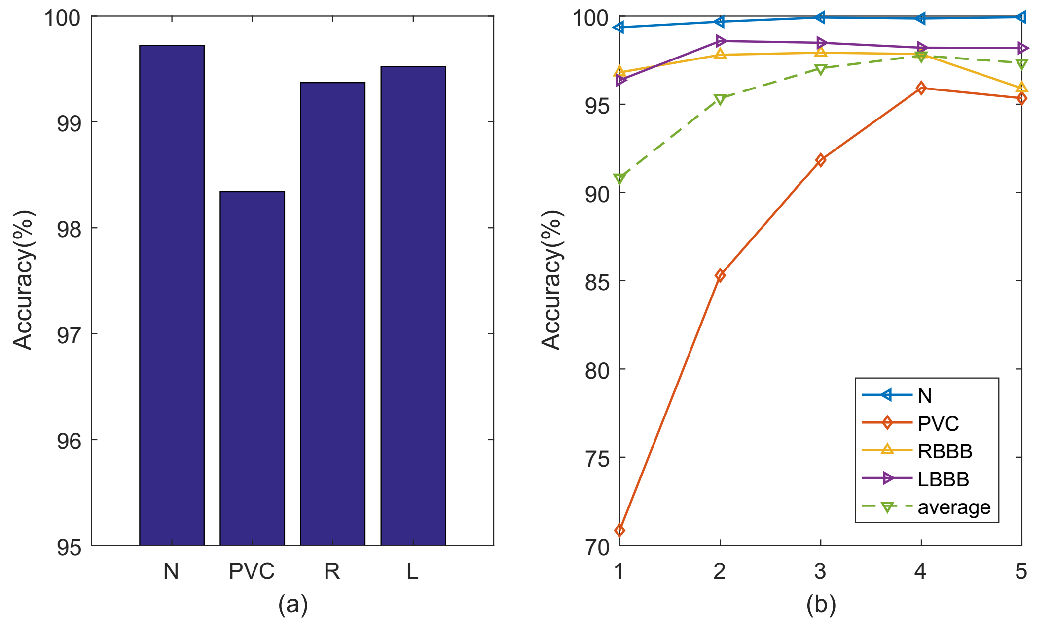
\includegraphics[width=9cm]{SVMAccuracy3.pdf}\\
	\caption{(a) Accuracy of the original signals under SVM method; (b) Compressed signals accuracy of different $q$ under SVM method}
	\label{SVMAccuracy1}
\end{figure}

\subsection{Performance of CNN Methods}
Table 3 and Figure 7(a) show the classification effect of the original signal under CNN method where 9939 in 10,000 training samples are correctly classified, and the average accuracy rate is 99.39\%. Among all categories, the accuracy of N beat is the highest, which is 99.88\% while that of  the PVC beat is the lowest, which is 98.92\%.

 \begin{center}
 \scriptsize
 %\begin{threeparttable}
 { Table~3 Accuracy of the Original Signals under CNN}\\
 \label{tab:3} \vskip 3pt
 \begin{tabular}{c|cc|c}
  \toprule
 Labels & Correct Number & Error Number & Test accuracy(\%)  \\
  \midrule
N    & 2449 & 3  & 99.88    \\
PVC  & 2479 & 27 & 98.92  \\
RBBB & 2555 & 7 & 99.73  \\
LBBB & 2456 & 24  & 99.03  \\
  \midrule
Total& 9939 & 61 & 99.39  \\
  \bottomrule
 \end{tabular}
\end{center}

As in Figure 6(b), Figure 7(b) shows the effect of different q on each accuracy. It can be seen that each recognition accuracy of N, RBBB and LBBB beats is above 95\%, and there is no significant downward trend with the decrease of the singular value $q$. However, only when the $q$ is greater than 4, the accuracy of PVC is more than 95\%, same as SVM method, the accuracy of PVC beat is increased with the increase of q.

\subsection{Evaluation}
The results of SVM and CNN have some similarities with each other: changes of q value have no obvious influence on the accuracy of N, RBBB and LBBB, and can maintain a high accuracy rate which is higher than 95\%. In both methods, $q$ has a significant impact on the accuracy of PVC beat. However, when $q\geq4$, the accuracy of PVC beat in both methods can be more than 95\%. Therefore, it can be concluded that the lossy compression of ECG signals can still achieve a high accuracy as long as  the appropriate $q$ is obtained.

\begin{figure}
	\centering
	% Requires \usepackage{graphicx}
	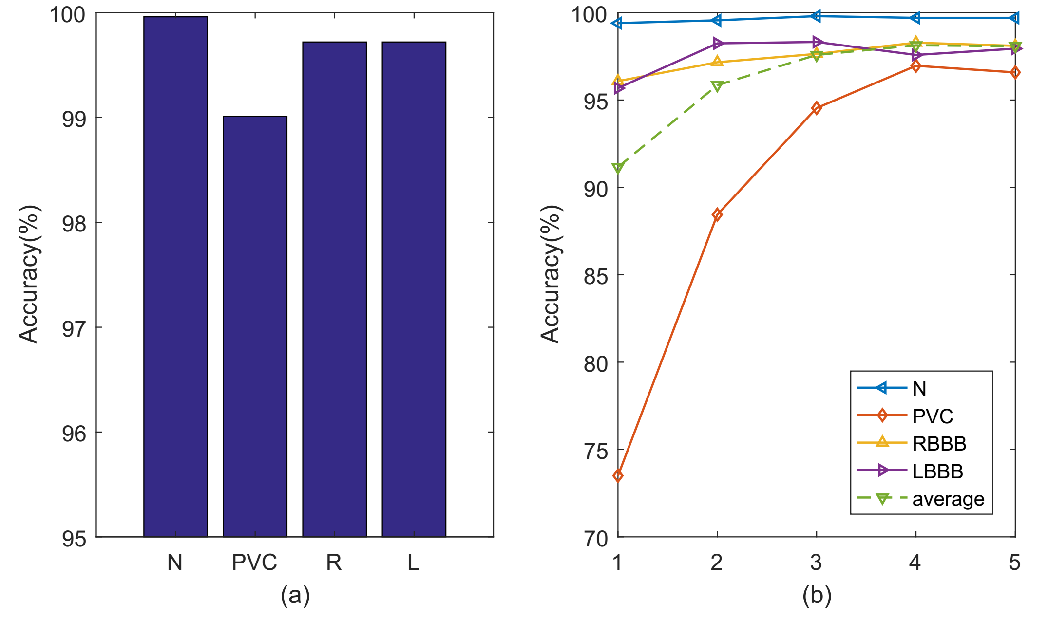
\includegraphics[width=9cm]{CNNAccuracy3.pdf}\\
	\caption{(a) Accuracy of the original signals under CNN method; (b) Compressed signals accuracy of different $q$ under CNN method}
	\label{CNNAccuracy1}
\end{figure}

\section{Multi-objective Optimization }
The previous section confirmed that when $q\succ4$, all the four types of compressed beats have satisfactory accuracy. Two factors, that is, CR and accuracy have to be considered to choose an appropriate value of $q$. If a higher accuracy is needed, $q$ should at least equal 4 or even larger while a more efficient transferring rate is needed, q should be smaller than 4, which of course will compromise the accuracy of PVC beat classification. This section describes how to use multi-objective optimization to select the appropriate parameters $q$ for different application scenarios.

\subsection{Fundamental methods}
Goal programming provides an optimization method to deal with two (or more than two) conflicting objectives and is widely used in mathematics, information theory and engineering. Instead of finding solutions which absolutely minimize or maximize objective functions, the task of goal programming is to find solutions that, if possible, satisfy a set of goals, or otherwise violate the goals minimally. This makes the approach more appealing to practical designers, compared to other optimization methods (e.g., linear programming models). The goal can be described as follow:
\begin{eqnarray}
&&
{\rm Minimize}\quad
\mathcal{O}\equiv \eta_{1}\delta_{1}^{-} + \eta_{2}\delta_{2}^{+},
 \nonumber \\
&&
{\rm subject\,\,to}\,
\left\{
\begin{array}{l}
\mathcal{C}(\vec{x})-\delta_{1}^{+}+\delta_{1}^{-} = \Delta_{C} \\
\mathcal{A}(\vec{x})-\delta_{2}^{+}+\delta_{2}^{-} = \Delta_{A} \\
\delta_{1}^{\pm},\delta_{2}^{\pm} \ge 0
%\\
%\vec{x}=(t\Omega/2\pi, k\Omega) \in \mathcal{M}
\end{array}
\right. .
\label{GP}
\end{eqnarray}
The weight factors $\eta_{1}$ and $\eta_{2}$ are given positive number, and represent the relative priority of objectives. If $\eta_{2} > \eta_{1}$, the condition for the error is prior to the one for the CR, and vice versa. The condition for the CR ($\mathcal{C} \geq \Delta_{C}$) is reformulated by the relation \( \mathcal{C} +\delta_{1}^{+}-\delta_{1}^{-} = \Delta_{C} \), with the deviations between the admissible error and the actual value, $\delta_{1}^{+}$ and $\delta_{1}^{-}$. When $\mathcal{C} > \Delta_{C}$ ($\mathcal{C} \le \Delta_{C}$), we set $\delta_{1}^{+}=\mathcal{C}-\Delta_{C}$ and $\delta_{1}^{-}=0$ ($\delta_{1}^{+}=0$ and $\delta_{1}^{-}=\Delta_{C}-\mathcal{C}$). Similarly, we can set $\delta_{2}^{\pm}$ via $\mathcal{A}-\delta_{2}^{+}+\delta_{2}^{-}=\Delta_{A}$. The smaller $\mathcal{O}$, the better performance of the measurement scenario. The minimum value of $\mathcal{O}$ corresponds to the best solution.

%\begin{figure}
%\setlength{\abovecaptionskip}{7pt}
%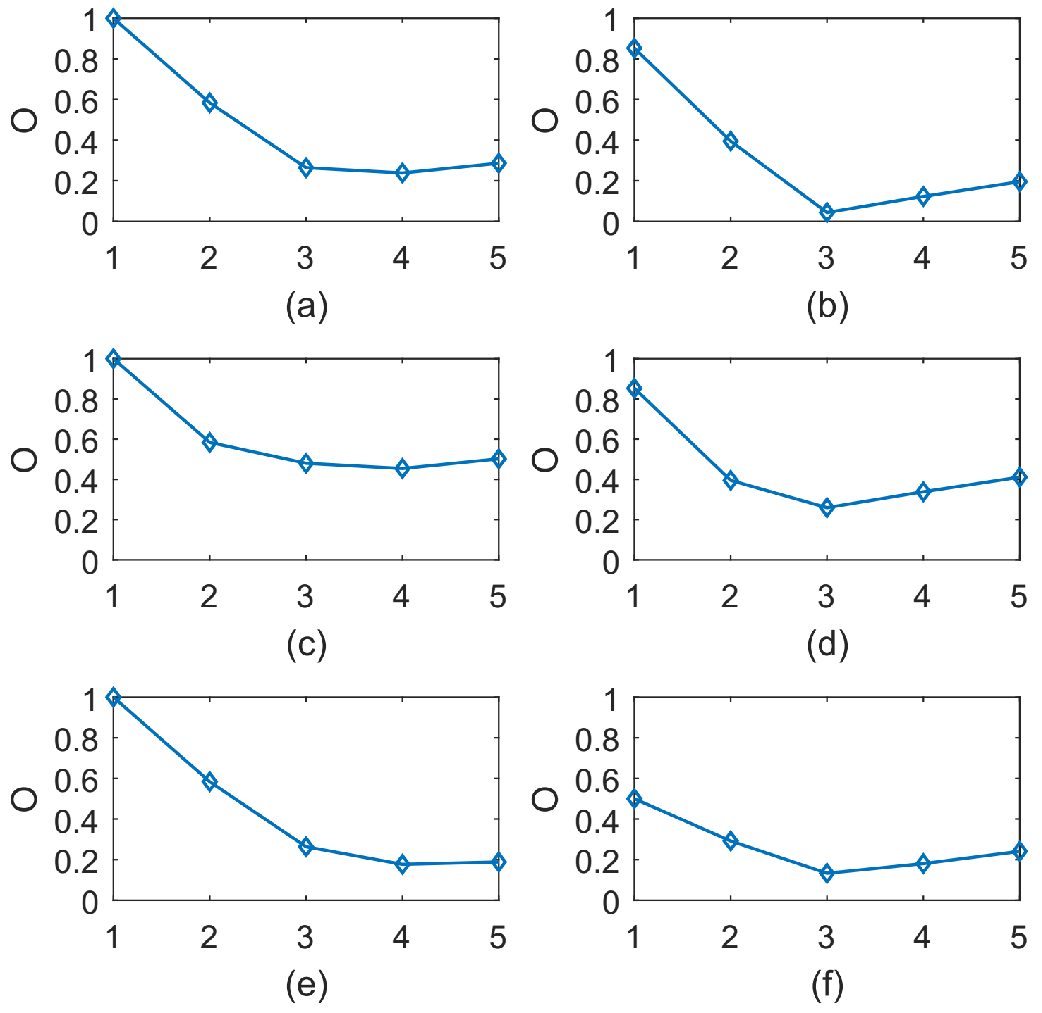
\includegraphics[width=1\columnwidth]{multobjectSVM}
%\caption{Value of the optimization function $\mathcal{O}$ in the goal programming model for several cases under SVM:
%(a) $\eta_1=\eta_2=1$ and $\Delta_C=90,\Delta_A=0.05$; (b) $\eta_1=\eta_2=1$ and $\Delta_C=90,\Delta_A=0.07$;
%(c) $\eta_1=\eta_2=1$ and $\Delta_C=130,\Delta_A=0.05$; (d) $\eta_1=\eta_2=1$ and $\Delta_C=130,\Delta_A=0.07$;
%(e) $\eta_1=0.5,\eta_2=1$ and $\Delta_C=90,\Delta_A=0.05$; (f) $\eta_1=1,\eta_2=0.5$ and $\Delta_C=90,\Delta_A=0.05$.}
%\end{figure}
%
%\begin{figure}
%\setlength{\abovecaptionskip}{7pt}
%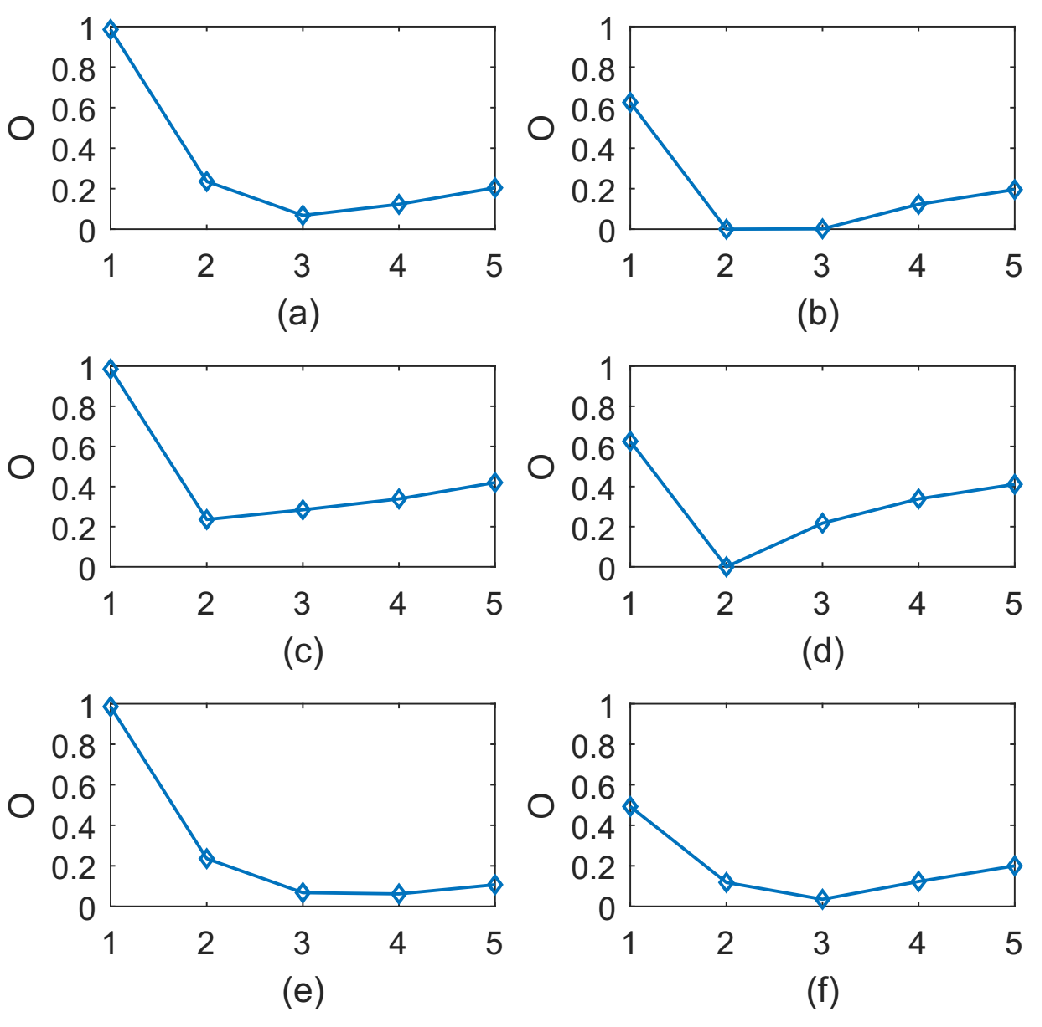
\includegraphics[width=1\columnwidth]{multobjectCNN}
%\caption{Value of the optimization function $\mathcal{O}$ in the goal programming model for several cases under CNN:
%(a) $\eta_1=\eta_2=1$ and $\Delta_C=90,\Delta_A=0.03$; (b) $\eta_1=\eta_2=1$ and $\Delta_C=90,\Delta_A=0.05$;
%(c) $\eta_1=\eta_2=1$ and $\Delta_C=130,\Delta_A=0.03$; (d) $\eta_1=\eta_2=1$ and $\Delta_C=130,\Delta_A=0.05$;
%(e) $\eta_1=0.5,\eta_2=1$ and $\Delta_C=90,\Delta_A=0.03$; (f) $\eta_1=1,\eta_2=0.5$ and $\Delta_C=90,\Delta_A=0.03$.}
%\end{figure}
\subsection{Experiment Procedure after Classification}
The results in Section 4 indicate a clear trade-off relationship between accuracy and the value of CR in ECG compression and transmission, which can be examined via a sophisticated method, multi-objective optimization or goal programming[27]. More specifically, let $\mathcal{C}$ be the CR and $\mathcal{A}$ be the average accuracy. We consider the multi-objective optimization such that $\mathcal{C} \geq \Delta_{C}$ and $\mathcal{A} \le \Delta_{A}$ for given (small) positive constants $\Delta_{C}$ and $\Delta_{A}$. The two parameters $\Delta C$ and $\Delta A$ are regarded as, admissible CR and permissible error respectively. Thus, a good measurement scenario can be obtained to increase the CR (i.e., maximize $\mathcal{C}$) while deminishing the error (i.e.,minimizing $\mathcal{A}$).

%The ultimate goal is to obtain a value of $q$, corresponding to a pair of $\Delta_{C}$ and $\Delta_{A}$ which lead to a satisfying and optimized compression and classification performance. By calculating the $max \frac{\Delta_{C}}{\Delta_{A}}$of each singular value, the maximum one is chosen and the corresponding $q$ is the optimal solution we want, which can be described as below:
%\begin{equation}
%q=\mathop{\arg\max}_{i} max (\frac{\Delta_{C_i}}{\Delta_{A_i}}),i=1,2,3,4,5
%\end{equation}

We use the average error rate obtained under the CNN method to represent $A$ and CR to represent $C$. $\Delta_{A}$ and $\Delta_{C}$ represent the ideal error rate and compression for different application scenarios respectively, while $\eta_{1}$ and $\eta_{2}$ represent the weights of $\Delta_{A}$ and $\Delta_{A}$, respectively. Figure 8 shows the optimization results for different parameters. The abscissa represents the number of singular values $q$, and the ordinate represents the value of the multi-objective function $O$. As can be seen from the above, the optimal result is when $q$ minimizes$O$. Figures 8(a) and (b) show the ideal parameter requirements for different scenarios. Figure 8(a) shows the need for a lower error rate where parameters are chosen as $\Delta_{A}$ =2\% and $\Delta_{C}$=75, and optimal result is $q=4$; Figure (b) shows that a requirement for a higher compression ratio where parameters are selected as $\Delta_{A}$=3\% and $\Delta_{C}$=90, and the optimal result is $q=3$.

\begin{figure}
	\centering
	% Requires \usepackage{graphicx}
	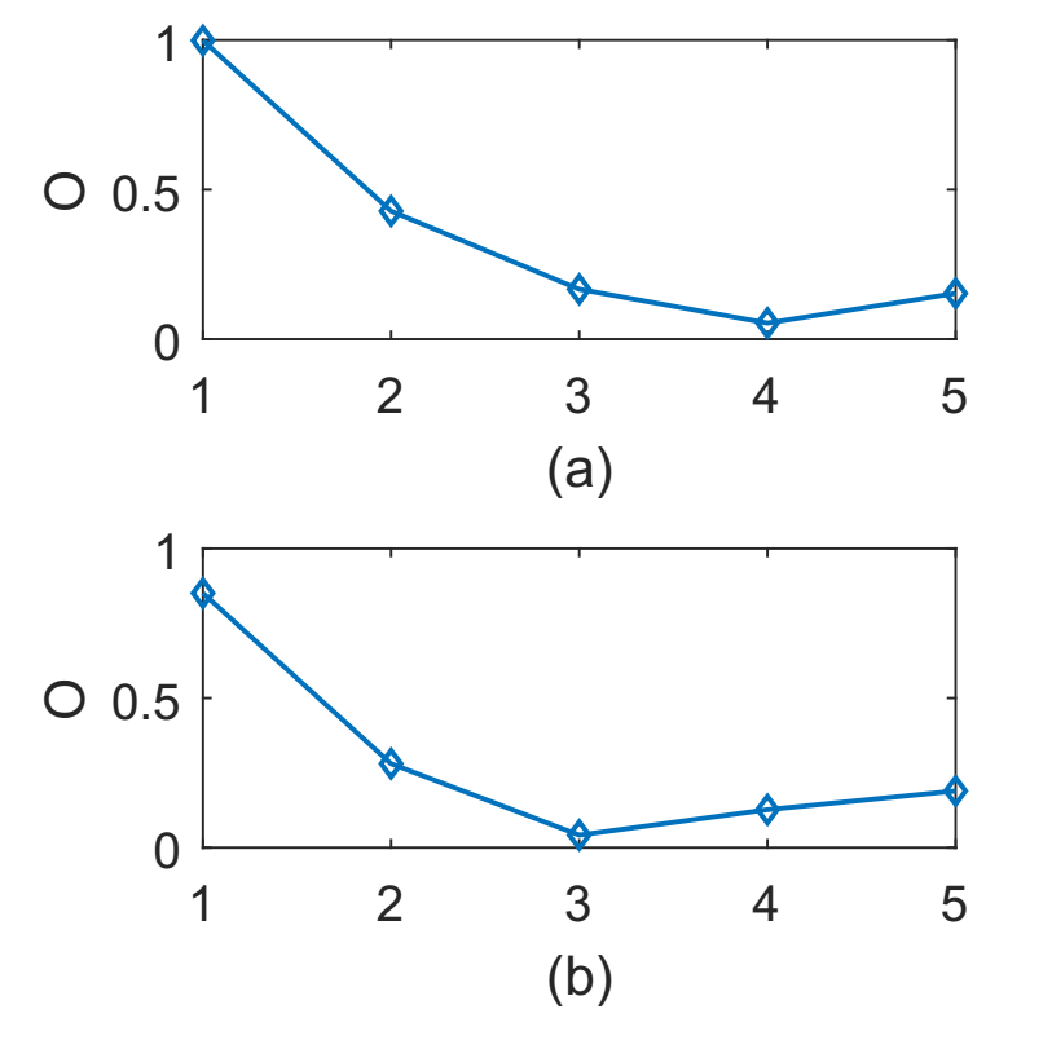
\includegraphics[width=6.5cm]{goal.pdf}\\
	\caption{(a) Optimization results under different parameters: (a)$\Delta_{A}$ = 2\%, $\Delta_{C}$ = 75, $\eta_{1} = \eta_{2}=1$; (b) $\Delta_{A}$ = 3\%, $\Delta_{C}$ = 90, $\eta_{1} = \eta_{2} =1$
}
	\label{CNNq2}
\end{figure}
According to requirements under different scenes, the most suitable $q$ can be gained by optimization.

\section{Conclusion}
In this paper, the SVD technology is used to compress and reconstruct the ECG signal. The obtained compressed ECG signals are then classified and detected using two kinds of methods for classification. Based on the experimental results, we have found that even if some information is lost, that is the quality of reconstructed signal is low, satisfying and high-quality classification result can be achieved in the lossy compression under the appropriate classifier as well as singular value. This result reduces the need for high-quality data compression in the field of ECG signal classification, thus simplifying the complexity of the problem. Furthermore, with the Error Rate and Compression Ratio as objective functions, multi-objective optimization method is introduced to choose the most appropriate $q$ in different application scenarios.


\vskip 12pt
{\fontsize{7.8pt}{9.4pt}\selectfont
	\begin{thebibliography}{99} \vskip 7pt
		\setlength{\parskip}{-2pt}
		

		%1
		\bibitem{1}A.Darwish, A.E.Hassanien, ``Wearable and implantable wireless sensor network solutions for healthcare monitoring,'' Sensors, vol. 12, no. 9, pp. 12375-12376, Sep. 2012.

		%2
		\bibitem{2}A. Kampouraki, G. Manis and C. Nikou, ``Heartbeat Time Series Classification With Support Vector Machines,'' IEEE Transactions on Information Technology in Biomedicine, vol. 13, no. 4, pp. 512-518, Jul. 2009.

		%3
		\bibitem{3}F. Melgani and Y. Bazi, ``Classification of Electrocardiogram Signals With Support Vector Machines and Particle Swarm Optimization,'' IEEE Transactions on Information Technology in Biomedicine, vol. 12, no. 5, pp. 667-677, Sep. 2008.

		%4
		\bibitem{4}Y.Li, W.Cui, ``Identifying the mislabeled training samples of ECG signals using machine learning,'' Biomedical Signal Processing and Control, vol. 47, pp. 168-176, Jan. 2019.

		%5
		\bibitem{5}L.Wang, G.Z.Yang, J.Huang, J.Zhang, L.Yu, Z.Nie, D.R.S.Cumming, ``A Wireless Biomedical Signal Interface System-on-Chip for Body Sensor Networks,'' IEEE Transactions on Biomedical Circuits and Systems, vol. 4, no. 2 pp. 112-117, Apr. 2010.

        %6
		\bibitem{6}J. Ma, T. Zhang and M. Dong, ``A Novel ECG Data Compression Method Using Adaptive Fourier Decomposition With Security Guarantee in e-Health Applications,'' IEEE Journal of Biomedical and Health Informatics, vol. 19, no. 3, pp. 986-994, Sep. 2015.

		%7
		\bibitem{7}J. R. Cox, F. M. Nolle, H. A. Fozzard and G. C. Oliver, ``AZTEC, a Preprocessing Program for Real-Time ECG Rhythm Analysis,'' IEEE Transactions on Biomedical Engineering, vol. BME-15, no. 2, pp. 128-129, April 1968.

		%8
		\bibitem{8}M.Ishijima, S.B.Shin, G.H.Hostetter, and J.Sklansky, ``Scan-Along Polygonal Approximation for Data Compression of Electrocardiograms,'' IEEE Transactions on Biomedical Engineering, vol. BME-30, no. 11, pp. 723-729, Nov. 1983.

		%9
		\bibitem{9}J. P. Abenstein and W. J. Tompkins, ``A New Data-Reduction Algorithm for Real-Time ECG Analysis,'' IEEE Transactions on Biomedical Engineering, vol. BME-29, no. 1, pp. 43-48, Jan. 1982.		


		%10	      	
		\bibitem{10}A. Al-Shrouf, M. Abo-Zahhad and S. M. Ahmed, ``A novel compression algorithm for electrocardiogram signals based on the linear prediction of the wavelet coefficients,'' Digital Signal Processing, vol. 13, no.4, pp. 604-622, Oct. 2003.

		%11		
		\bibitem{11}S. M. S. Jalaleddine, C. G. Hutchens, R. D. Strattan and W. A. Coberly, ``ECG data compression techniques-a unified approach,'' IEEE Transactions on Biomedical Engineering, vol. 37, no. 4, pp. 329-343, Apr. 1990.

		%12        unfinish
		\bibitem{12}R.W.McCaughern, A.M.Rosie, and F.C.Monds, ``Asynchronous data compression techniques,'' in Proc. Purdue Centennial Year Symp. Inf. Process., 1969, vol. 2, pp. 525-531.

		%13
		\bibitem{13}B. R. S. Reddy and I. S. N. Murthy, ``ECG Data Compression Using Fourier Descriptors,'' IEEE Transactions on Biomedical Engineering, vol. BME-33, no. 4, pp. 428-434, Apr. 1986.

		%14
		\bibitem{14}S. Olmos, M. Millan, J. Garcia and P. Laguna, ``ECG data compression with the Karhunen-Loeve transform,'' Computers in Cardiology 1996, Indianapolis, IN, USA, 1996, pp. 253-256.

		%15
		\bibitem{15}L.V.Batista, E.U.Kurt Melcher, and L.C.Carvalho, ``Compression of ECG signals by optimized quantization of discrete cosine transform coefficients,'' Med. Eng. Phys., vol. 23, no.2, pp. 127-134, Mar. 2001.

		%16
		\bibitem{16}M.L.Hilton, ``Wavelet and wavelet packet compression of electrocardiograms,'' IEEE Trans. Biomed. Eng., vol. 44, no. 5, pp. 394-402, May 1997.

		%17
		\bibitem{17}J.Wei, C.Chang, N.Chou, and G.Jan, ``ECG data compression using truncated singular value decomposition,'' IEEE Transactions on Information Technology in Biomedicine, vol. 5, no. 4, pp. 290-299, Dec. 2001.

		%18
		\bibitem{18}S.Padhy, L.N.Sharma, and S.Dandapat, ``Multilead ECG data compression using SVD in multiresolution domain,'' Biomedical Signal Processing and Control, vol. 23, no. 2, pp. 10-18, Jan. 2016.

		%19
		\bibitem{19}K. Duda, P. Turcza and T. P. Zielinski, ``Lossless ECG Compression with Lifting Wavelet Transform,'' Instrument and Measurement Technology Conference, 2001, pp. 640-644.

		%20
		\bibitem{20}E. D. Ubeyli, ``Detecting variabilities of ECG signals by Lyapunov exponents,'' Neural Computing and Applications, vol. 18, no. 7, pp. 653-662, Oct. 2009.

        %21
		\bibitem{21}Adolf Grauel, Lars A.Ludwig, Georg Klene, ``ECG Diagnostics by Fuzzy Decision Making[J],'' International Journal of Uncertainty, Fuzziness and Knowledge-Based Systems, vol. 6, no. 2, pp. 201-210, Apr. 1998.

		%22
		\bibitem{22}K. Shojaian, R. Amirfatahi, F. Kolahdouzan, ``Detection of Acute Atrial-Ventricular Arrhythmias Based on ECG Delineator: Evaluation on MIT/BIH Standard Databases[J],'' Majlesi Journal of Electrical Engineering, vol. 2, no. 1, pp 1-10, 2008.

        %23
		\bibitem{23}T. Y. Liu, K. J. Lin and H. C. Wu, ``ECG Data Encryption Then Compression Using Singular Value Decomposition[J],'' IEEE Journal of Biomedical and Health Informatics, vol. 22, no. 3, pp. 707-713, May. 2018.

        %24
		\bibitem{24}Y. Lecun, Y. Bengio and G. Hinton, ``Deep learning,'' Nature, vol. 521, no. 7553, pp. 436-444, Mar. 2015.

        %25
		\bibitem{25}Y. Boureau, N. Le Roux, F. Bach, J. Ponce and Y. LeCun, ``Ask the locals: Multi-way local pooling for image recognition,'' 2011 International Conference on Computer Vision, Barcelona, Nov. 2011, pp. 2651-2658.

        %26
		\bibitem{26}Y. Wang, C. J. Deepu and Y. Lian, ``A computationally efficient QRS detection algorithm for wearable ECG sensors,'' 2011 Annual International Conference of the IEEE Engineering in Medicine and Biology Society, Boston, MA, 2011, pp. 5641-5644.
        %27
        \bibitem{27}M. J. Schniederjans,c``Goal Programming: Methodology and Applications,'' (Kluwer, Boston, 1995).
        %28
        \bibitem{28}https://commons.wikimedia.org/wiki/File:SinusRhythmLabels.svg
        %29
        \bibitem{29}Y. Lecun et al, ``Gradient-based learning applied to document recognition,'' Proceedings of the IEEE, vol. 86, no. 11, pp. 2278-2324, Nov. 1998.


\end{thebibliography}}

\end{document}


